\section{Additional results}
\label{app:more}

\subsection{Full method tables and confidence intervals}
\label{app:more-tables}

\Cref{tab:compas,tab:learning} give the full method lists behind
\cref{tab:main}, including observed AUROC and the imputation baseline;
\cref{tab:compas-ci,tab:learning-ci} give the half-widths of the 95\%
confidence intervals ($t$-based) for the two metrics the text compares, and
\cref{fig:learning} plots realised risk against certified regret.

\begin{table*}[h]
\centering\small
\caption{\textbf{Methods on COMPAS} --- real release decisions, recorded
censored outcomes, out of sample, $\nExpSixSeeds$ splits (mean; 95\% CIs in
\cref{app:more-tables}). Certificates are evaluated at $\Gamma=\nCompasOR$,
the recorded detained-versus-released odds ratio. Heckman is shown as the
range over splits.}
\label{tab:compas}
\begin{tabular}{lccccc}
\toprule
method & risk $\downarrow$ & AUROC $\uparrow$ & obs.\ AUROC & w.c.\ risk $\downarrow$ & regret $\downarrow$\\
\midrule
ERM-observed  & $\nCompasMErmRisk$ & $\nCompasMErmAuroc$ & $\nCompasMErmObsAuroc$ & $\nCompasMErmWc$ & $\nCompasMErmRegret$\\
IPW           & $\nCompasMIpwRisk$ & $\nCompasMIpwAuroc$ & $\nCompasMIpwObsAuroc$ & $\nCompasMIpwWc$ & $\nCompasMIpwRegret$\\
AIPW          & $\nCompasMAipwRisk$ & $\nCompasMAipwAuroc$ & $\nCompasMAipwObsAuroc$ & $\nCompasMAipwWc$ & $\nCompasMAipwRegret$\\
Imputation    & $\nCompasMImpRisk$ & $\nCompasMImpAuroc$ & $\nCompasMImpObsAuroc$ & $\nCompasMImpWc$ & $\nCompasMImpRegret$\\
Heckman probit & $\nCompasMHeckmanRiskMin$--$\nCompasMHeckmanRiskMax$ & $\nCompasMHeckmanAurocMin$--$\nCompasMHeckmanAurocMax$ & --- & $\nCompasMHeckmanWcMin$--$\nCompasMHeckmanWcMax$ & $\nCompasMHeckmanRegretMin$--$\nCompasMHeckmanRegretMax$\\
Manski ($\Gamma=\infty$) & $\nCompasMManskiRisk$ & $\nCompasMManskiAuroc$ & $\nCompasMManskiObsAuroc$ & $\nCompasMManskiWc$ & $\nCompasMManskiRegret$\\
DCL, minimax risk   & $\nCompasMDclTwoRisk$ & $\nCompasMDclTwoAuroc$ & $\nCompasMDclTwoObsAuroc$ & $\mathbf{\nCompasMDclTwoWc}$ & $\nCompasMDclTwoRegret$\\
DCL, minimax regret & $\mathbf{\nCompasMDclRegTwoRisk}$ & $\nCompasMDclRegTwoAuroc$ & $\nCompasMDclRegTwoObsAuroc$ & $\nCompasMDclRegTwoWc$ & $\mathbf{\nCompasMDclRegTwoRegret}$\\
\emph{oracle (uncensored)} & \emph{$\nCompasMOracleRisk$} & \emph{$\nCompasMOracleAuroc$} & --- & \emph{$\nCompasMOracleWc$} & \emph{$\nCompasMOracleRegret$}\\
\bottomrule
\end{tabular}
\end{table*}

\begin{table*}[h]
\centering\small
\caption{\textbf{Out-of-sample deployment metrics and certificates}, mean over
$\nExpTwoSeeds$ seeds (95\% CIs in \cref{app:more-tables}). \emph{Risk} and
\emph{AUROC} are on the complete outcomes of \emph{all} units; \emph{observed
AUROC} is what a practitioner would report; \emph{worst-case risk} and
\emph{regret} are certified at the instance's $\Gamma_0$
($\nExpTwoLendingGammaZero$ and $\nExpTwoSlBenchGammaZero$). Best in each
column in bold; the oracle is not attainable.}
\label{tab:learning}
\begin{tabular}{llccccc}
\toprule
& method & risk $\downarrow$ & AUROC $\uparrow$ & obs.\ AUROC & w.c.\ risk $\downarrow$ & regret $\downarrow$\\
\midrule
\multirow{7}{*}{\rotatebox{90}{Lending Club}}
& ERM-observed        & $\nExpTwoLendingErmRisk$ & $\nExpTwoLendingErmAuroc$ & $\nExpTwoLendingErmObsAuroc$ & $\nExpTwoLendingErmWc$ & $\nExpTwoLendingErmRegret$\\
& IPW                 & $\nExpTwoLendingIpwRisk$ & $\nExpTwoLendingIpwAuroc$ & $\nExpTwoLendingIpwObsAuroc$ & $\nExpTwoLendingIpwWc$ & $\nExpTwoLendingIpwRegret$\\
& AIPW                & $\nExpTwoLendingAipwRisk$ & $\nExpTwoLendingAipwAuroc$ & $\nExpTwoLendingAipwObsAuroc$ & $\nExpTwoLendingAipwWc$ & $\nExpTwoLendingAipwRegret$\\
& Heckman probit      & $\nExpTwoLendingHeckmanRisk$ & $\mathbf{\nExpTwoLendingHeckmanAuroc}$ & $\nExpTwoLendingHeckmanObsAuroc$ & $\nExpTwoLendingHeckmanWc$ & $\nExpTwoLendingHeckmanRegret$\\
& DCL, minimax risk   & $\nExpTwoLendingDclTwoRisk$ & $\nExpTwoLendingDclTwoAuroc$ & $\nExpTwoLendingDclTwoObsAuroc$ & $\mathbf{\nExpTwoLendingDclTwoWc}$ & $\nExpTwoLendingDclTwoRegret$\\
& DCL, minimax regret & $\mathbf{\nExpTwoLendingDclRegTwoRisk}$ & $\nExpTwoLendingDclRegTwoAuroc$ & $\nExpTwoLendingDclRegTwoObsAuroc$ & $\nExpTwoLendingDclRegTwoWc$ & $\mathbf{\nExpTwoLendingDclRegTwoRegret}$\\
& \emph{oracle}       & \emph{$\nExpTwoLendingOracleRisk$} & \emph{$\nExpTwoLendingOracleAuroc$} & --- & \emph{$\nExpTwoLendingOracleWc$} & \emph{$\nExpTwoLendingOracleRegret$}\\
\midrule
\multirow{7}{*}{\rotatebox{90}{SL-Bench}}
& ERM-observed        & $\nExpTwoSlBenchErmRisk$ & $\nExpTwoSlBenchErmAuroc$ & $\nExpTwoSlBenchErmObsAuroc$ & $\nExpTwoSlBenchErmWc$ & $\nExpTwoSlBenchErmRegret$\\
& IPW                 & $\nExpTwoSlBenchIpwRisk$ & $\nExpTwoSlBenchIpwAuroc$ & $\nExpTwoSlBenchIpwObsAuroc$ & $\nExpTwoSlBenchIpwWc$ & $\nExpTwoSlBenchIpwRegret$\\
& AIPW                & $\nExpTwoSlBenchAipwRisk$ & $\nExpTwoSlBenchAipwAuroc$ & $\nExpTwoSlBenchAipwObsAuroc$ & $\nExpTwoSlBenchAipwWc$ & $\nExpTwoSlBenchAipwRegret$\\
& Heckman probit      & $\mathbf{\nExpTwoSlBenchHeckmanRisk}$ & $\mathbf{\nExpTwoSlBenchHeckmanAuroc}$ & $\nExpTwoSlBenchHeckmanObsAuroc$ & $\nExpTwoSlBenchHeckmanWc$ & $\nExpTwoSlBenchHeckmanRegret$\\
& DCL, minimax risk   & $\nExpTwoSlBenchDclThreeRisk$ & $\nExpTwoSlBenchDclThreeAuroc$ & $\nExpTwoSlBenchDclThreeObsAuroc$ & $\mathbf{\nExpTwoSlBenchDclThreeWc}$ & $\nExpTwoSlBenchDclThreeRegret$\\
& DCL, minimax regret & $\nExpTwoSlBenchDclRegThreeRisk$ & $\nExpTwoSlBenchDclRegThreeAuroc$ & $\nExpTwoSlBenchDclRegThreeObsAuroc$ & $\nExpTwoSlBenchDclRegThreeWc$ & $\mathbf{\nExpTwoSlBenchDclRegThreeRegret}$\\
& \emph{oracle}       & \emph{$\nExpTwoSlBenchOracleRisk$} & \emph{$\nExpTwoSlBenchOracleAuroc$} & --- & \emph{$\nExpTwoSlBenchOracleWc$} & \emph{$\nExpTwoSlBenchOracleRegret$}\\
\bottomrule
\end{tabular}
\end{table*}

\begin{figure}[h]
\centering
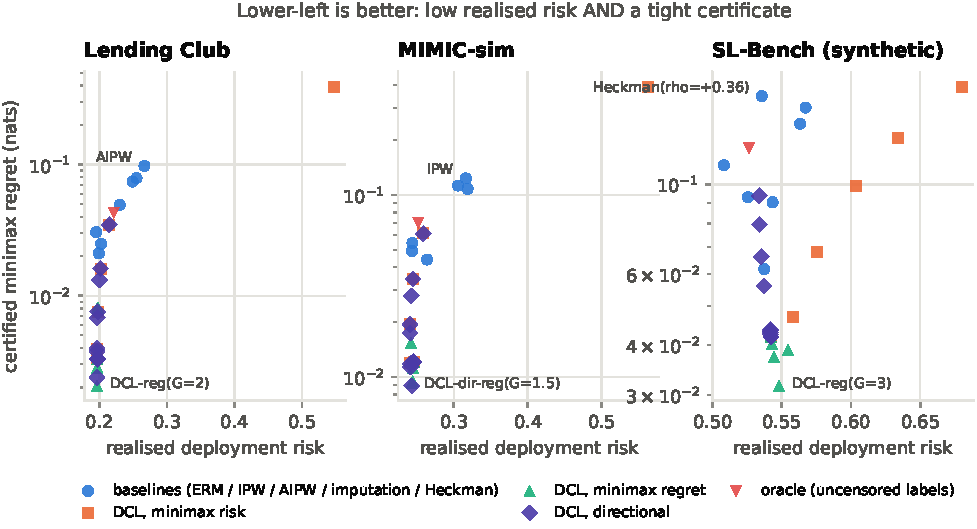
\includegraphics[width=\linewidth]{figures/fig3_learning}
\caption{\textbf{Realised deployment risk against certified minimax regret}
(log scale). Each point is a method; DCL variants are shown at several
$\Gamma$. The minimax-regret rule occupies the lower-left corner on every
testbed.}
\label{fig:learning}
\end{figure}

\begin{table*}[h]
\centering\small
\caption{COMPAS (recorded outcome): realised risk and certified regret with
95\% CIs over $\nExpSixSeeds$ splits.}
\label{tab:compas-ci}
\begin{tabular}{lcc}
\toprule
method & risk & regret\\
\midrule
ERM-observed & $\nCompasMErmRisk\pm\nCompasMErmRiskCI$ & $\nCompasMErmRegret\pm\nCompasMErmRegretCI$\\
IPW & $\nCompasMIpwRisk\pm\nCompasMIpwRiskCI$ & $\nCompasMIpwRegret\pm\nCompasMIpwRegretCI$\\
AIPW & $\nCompasMAipwRisk\pm\nCompasMAipwRiskCI$ & $\nCompasMAipwRegret\pm\nCompasMAipwRegretCI$\\
Imputation & $\nCompasMImpRisk\pm\nCompasMImpRiskCI$ & $\nCompasMImpRegret\pm\nCompasMImpRegretCI$\\
Heckman probit & $\nCompasMHeckmanRisk\pm\nCompasMHeckmanRiskCI$ & $\nCompasMHeckmanRegret\pm\nCompasMHeckmanRegretCI$\\
Manski & $\nCompasMManskiRisk\pm\nCompasMManskiRiskCI$ & $\nCompasMManskiRegret\pm\nCompasMManskiRegretCI$\\
DCL, minimax risk & $\nCompasMDclTwoRisk\pm\nCompasMDclTwoRiskCI$ & $\nCompasMDclTwoRegret\pm\nCompasMDclTwoRegretCI$\\
DCL, minimax regret & $\nCompasMDclRegTwoRisk\pm\nCompasMDclRegTwoRiskCI$ & $\nCompasMDclRegTwoRegret\pm\nCompasMDclRegTwoRegretCI$\\
oracle & $\nCompasMOracleRisk\pm\nCompasMOracleRiskCI$ & $\nCompasMOracleRegret\pm\nCompasMOracleRegretCI$\\
\bottomrule
\end{tabular}
\end{table*}

\begin{table*}[h]
\centering\small
\caption{Lending Club and SL-Bench: realised risk and certified regret with
95\% CIs over $\nExpTwoSeeds$ seeds.}
\label{tab:learning-ci}
\resizebox{\textwidth}{!}{\begin{tabular}{lcccc}
\toprule
 & \multicolumn{2}{c}{Lending Club} & \multicolumn{2}{c}{SL-Bench}\\
method & risk & regret & risk & regret\\
\midrule
ERM-observed & $\nExpTwoLendingErmRisk\pm\nExpTwoLendingErmRiskCI$ & $\nExpTwoLendingErmRegret\pm\nExpTwoLendingErmRegretCI$ & $\nExpTwoSlBenchErmRisk\pm\nExpTwoSlBenchErmRiskCI$ & $\nExpTwoSlBenchErmRegret\pm\nExpTwoSlBenchErmRegretCI$\\
IPW & $\nExpTwoLendingIpwRisk\pm\nExpTwoLendingIpwRiskCI$ & $\nExpTwoLendingIpwRegret\pm\nExpTwoLendingIpwRegretCI$ & $\nExpTwoSlBenchIpwRisk\pm\nExpTwoSlBenchIpwRiskCI$ & $\nExpTwoSlBenchIpwRegret\pm\nExpTwoSlBenchIpwRegretCI$\\
AIPW & $\nExpTwoLendingAipwRisk\pm\nExpTwoLendingAipwRiskCI$ & $\nExpTwoLendingAipwRegret\pm\nExpTwoLendingAipwRegretCI$ & $\nExpTwoSlBenchAipwRisk\pm\nExpTwoSlBenchAipwRiskCI$ & $\nExpTwoSlBenchAipwRegret\pm\nExpTwoSlBenchAipwRegretCI$\\
DCL, minimax risk & $\nExpTwoLendingDclTwoRisk\pm\nExpTwoLendingDclTwoRiskCI$ & $\nExpTwoLendingDclTwoRegret\pm\nExpTwoLendingDclTwoRegretCI$ & $\nExpTwoSlBenchDclThreeRisk\pm\nExpTwoSlBenchDclThreeRiskCI$ & $\nExpTwoSlBenchDclThreeRegret\pm\nExpTwoSlBenchDclThreeRegretCI$\\
DCL, minimax regret & $\nExpTwoLendingDclRegTwoRisk\pm\nExpTwoLendingDclRegTwoRiskCI$ & $\nExpTwoLendingDclRegTwoRegret\pm\nExpTwoLendingDclRegTwoRegretCI$ & $\nExpTwoSlBenchDclRegThreeRisk\pm\nExpTwoSlBenchDclRegThreeRiskCI$ & $\nExpTwoSlBenchDclRegThreeRegret\pm\nExpTwoSlBenchDclRegThreeRegretCI$\\
oracle & $\nExpTwoLendingOracleRisk\pm\nExpTwoLendingOracleRiskCI$ & $\nExpTwoLendingOracleRegret\pm\nExpTwoLendingOracleRegretCI$ & $\nExpTwoSlBenchOracleRisk\pm\nExpTwoSlBenchOracleRiskCI$ & $\nExpTwoSlBenchOracleRegret\pm\nExpTwoSlBenchOracleRegretCI$\\
\bottomrule
\end{tabular}}
\end{table*}

\begin{figure}[h]
\centering
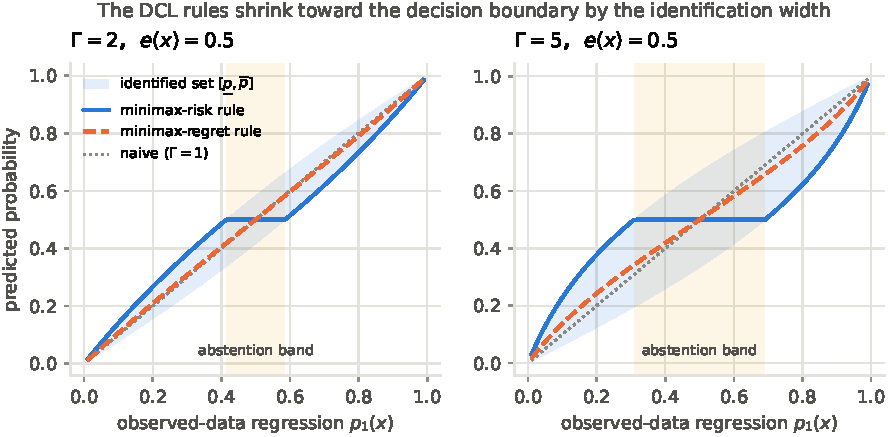
\includegraphics[width=0.7\linewidth]{figures/fig7_rules}
\caption{\textbf{The two closed-form DCL rules} (\cref{thm:dcl}(d) and
\cref{prop:regret}). Shaded: the identified set at $e(x)=0.5$. The
minimax-risk rule \eqref{eq:bayes-act} flattens to the decision boundary on
the abstention band; the minimax-regret rule \eqref{eq:regret-rule} stays
inside the identified set and remains a probability estimate throughout.}
\label{fig:rules}
\end{figure}

\subsection{COMPAS: lineage and time at risk}
\label{app:compas-audit}

\emph{Lineage.} ProPublica's \texttt{compas-scores-two-years.csv}
($n=\nCompasTarNRaw$) is filtered as in their analysis (screening within 30
days of arrest, ordinary-traffic offences and missing scores removed;
$n=\nCompasTarNPropublica$), then to units with jail dates and an index
custody spell of at most 180 days ($n=\nCompasTarNCohort$). $T=1$ is release
within two days of booking ($\nCompasTarSelectionPct$ of the cohort); the
median index custody is $\nCompasTarCustodyReleasedMedian$ days in the
released group and $\nCompasTarCustodyDetainedMedian$ days (90th percentile
$\nCompasTarCustodyDetainedQNinety$) in the detained group.

\emph{Time at risk.} Detention incapacitates: a defendant held for part of the
two-year window has less opportunity to be rearrested. ProPublica's survival
fields (\texttt{start}, \texttt{end}, \texttt{event}) give each unit's time
at risk in the community, so we also score \emph{rearrest within 730 days at
risk}, dropping units with neither an event nor 730 days of at-risk
follow-up ($\nCompasTarKeptPct$ kept; $\nCompasTarKeptDetainedPct$ of the
detained). The recorded detained/released rearrest rates are
$\nCompasTarPZeroRecorded$ vs.\ $\nCompasTarPOneRecorded$ (odds ratio
$\nCompasTarORRecorded$); with exposure held fixed they are
$\nCompasTarPZeroExposure$ vs.\ $\nCompasTarPOneExposure$ (odds ratio
$\nCompasTarORExposure$). The adjustment \emph{raises} the odds ratio:
incapacitation was masking selection on unobservables, not manufacturing it,
so the recorded anchor is, if anything, conservative. Under the
exposure-adjusted outcome the interval covers the recorded AUROC in
$\nCompasExpCovAtOR$ of splits at $\Gamma=\nCompasExpOR$ and in
$\nCompasExpCovAtOne$ at $\Gamma=1$; the minimax-regret rule's realised risk
is $\nCompasExpMDclRegTwoRisk\pm\nCompasExpMDclRegTwoRiskCI$ against ERM's
$\nCompasExpMErmRisk\pm\nCompasExpMErmRiskCI$ and the oracle's
$\nCompasExpMOracleRisk\pm\nCompasExpMOracleRiskCI$. Neither outcome is a
causal ground truth; both are recorded outcomes, and the paper's wording
follows that. The audit script is \texttt{audit/compas\_time\_at\_risk.py}.

\subsection{Lending Club: the hidden signal is kept out of $X$ by code}
\label{app:lending-guard}

The semi-synthetic construction is only meaningful if the underwriter's signal
$S$ (assigned interest rate and sub-grade) is absent from the learner's $X$.
\texttt{dcl.data.semisynthetic.assert\_hidden\_signal\_excluded} enforces this
at load time and raises otherwise: (i) no feature name matches the raw columns
$S$ is built from (\texttt{int\_rate}, \texttt{sub\_grade}, \texttt{grade});
(ii) no column of $X$ reproduces $S$ or a monotone transform of it (Pearson
and Spearman $|\rho|<0.95$ for every column); (iii) $S$ is not linearly
reconstructible from $X$ (in-sample $R^2<0.95$). The diagnostics are stored
with the dataset object and unit-tested (\texttt{tests/test\_data\_guards.py}).
The check guards against deterministic derivatives of $S$, not against
dependence between $S$ and $X$, which is expected and is what residualisation
removes before $\Gamma_0$ is calibrated.

\subsection{Falsification and misspecification tables}
\label{app:falsify}

\begin{table*}[h]
\centering\small
\caption{\textbf{Falsifying $\Gamma$ from leniency variation} (SL-Bench,
5 decision makers, $\nExpFourNCells$ configurations; each row averages the
leniency spreads). $\Gamma_0^{\mathrm{cond}}$ is the within-decision-maker
sensitivity parameter that \cref{prop:falsify} bounds from below;
``recovered'' is $\log\Gamma_{\min}/\log\Gamma_0^{\mathrm{cond}}$ at the
robust (95th percentile) variant.}
\label{tab:falsify}
\begin{tabular}{cccccc}
\toprule
target $\Gamma_0$ & reliance on $S$ & $\Gamma_0^{\mathrm{cond}}$ & $\Gamma_{\min}$ & $\Gamma_{\min}$ (q95) & recovered\\
\midrule
$1.0$ & homogeneous   & $\nExpFourOneHomGzCond$ & $\nExpFourOneHomGmin$ & $\nExpFourOneHomGminQ$ & ---\\
$1.0$ & heterogeneous & $\nExpFourOneHetGzCond$ & $\nExpFourOneHetGmin$ & $\nExpFourOneHetGminQ$ & ---\\
$1.5$ & homogeneous   & $\nExpFourOneFiveHomGzCond$ & $\nExpFourOneFiveHomGmin$ & $\nExpFourOneFiveHomGminQ$ & $\nExpFourOneFiveHomRec$\\
$1.5$ & heterogeneous & $\nExpFourOneFiveHetGzCond$ & $\nExpFourOneFiveHetGmin$ & $\nExpFourOneFiveHetGminQ$ & $\nExpFourOneFiveHetRec$\\
$2.0$ & homogeneous   & $\nExpFourTwoHomGzCond$ & $\nExpFourTwoHomGmin$ & $\nExpFourTwoHomGminQ$ & $\nExpFourTwoHomRec$\\
$2.0$ & heterogeneous & $\nExpFourTwoHetGzCond$ & $\nExpFourTwoHetGmin$ & $\nExpFourTwoHetGminQ$ & $\nExpFourTwoHetRec$\\
$3.0$ & homogeneous   & $\nExpFourThreeHomGzCond$ & $\nExpFourThreeHomGmin$ & $\nExpFourThreeHomGminQ$ & $\nExpFourThreeHomRec$\\
$3.0$ & heterogeneous & $\nExpFourThreeHetGzCond$ & $\nExpFourThreeHetGmin$ & $\nExpFourThreeHetGminQ$ & $\nExpFourThreeHetRec$\\
$5.0$ & homogeneous   & $\nExpFourFiveHomGzCond$ & $\nExpFourFiveHomGmin$ & $\nExpFourFiveHomGminQ$ & $\nExpFourFiveHomRec$\\
$5.0$ & heterogeneous & $\nExpFourFiveHetGzCond$ & $\nExpFourFiveHetGmin$ & $\nExpFourFiveHetGminQ$ & $\nExpFourFiveHetRec$\\
\bottomrule
\end{tabular}
\end{table*}

\begin{figure}[h]
\centering
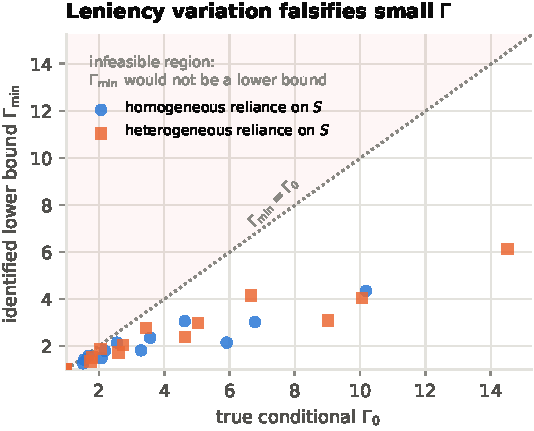
\includegraphics[width=0.5\linewidth]{figures/fig6_falsification}
\caption{\textbf{Every point lies below the diagonal:} the identified lower
bound never exceeds the true conditional $\Gamma_0$. Heterogeneous reliance on
private information loosens the bound, as \cref{prop:falsify}'s intersection
argument predicts.}
\label{fig:falsify}
\end{figure}

\label{app:misspec}
\emph{Misspecified $\Gamma$.} Over $\nExpFourMisSeeds$ seeds and a
$\nExpFourMisRange$-fold range of assumed $\Gamma$ on SL-Bench, coverage of the
deployment AUROC is $\nExpFourMisCovLow$ when $\Gamma\le\Gamma_0/2$ and
$\nExpFourMisCovHigh$ otherwise; the mean width rises monotonically from
$\nExpFourMisWidthMin$ at the smallest $\Gamma$ to $\nExpFourMisWidthMax$ at
the largest.

\subsection{Generalisation scaling}
\label{app:scaling}

\begin{table*}[h]
\centering\small
\caption{\textbf{Uniform deviation over the score class} --- the quantity
\cref{thm:generalization} bounds --- on SL-Bench, $\nExpFiveSeedsDev$ seeds per
cell. $B=B_0+\log\Gamma$ is the score range the class must reach to contain
the population optimum.}
\label{tab:scaling}
\begin{tabular}{lcccccc}
\toprule
$\Gamma$ & $1.5$ & $2$ & $3$ & $6$ & $12$ & $24$\\
\midrule
$B=B_0+\log\Gamma$ & $\nExpFiveOneFiveB$ & $\nExpFiveTwoB$ & $\nExpFiveThreeB$ & $\nExpFiveSixB$ & $\nExpFiveTwelveB$ & $\nExpFiveTwentyFourB$\\
rate exponent in $n$ & $\nExpFiveOneFiveRate$ & $\nExpFiveTwoRate$ & $\nExpFiveThreeRate$ & $\nExpFiveSixRate$ & $\nExpFiveTwelveRate$ & $\nExpFiveTwentyFourRate$\\
coefficient of $n^{-1/2}$ & $\nExpFiveOneFiveCoef$ & $\nExpFiveTwoCoef$ & $\nExpFiveThreeCoef$ & $\nExpFiveSixCoef$ & $\nExpFiveTwelveCoef$ & $\nExpFiveTwentyFourCoef$\\
\bottomrule
\end{tabular}
\end{table*}

\begin{figure}[h]
\centering
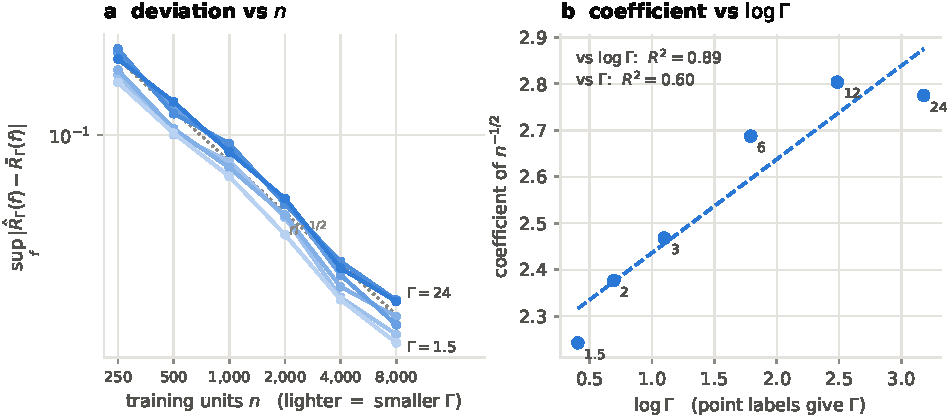
\includegraphics[width=0.8\linewidth]{figures/fig5_generalization}
\caption{\textbf{The generalisation bound in practice}
(\cref{thm:generalization}). (a) The uniform deviation decays at $n^{-1/2}$
for every $\Gamma$ (light to dark). (b) Its coefficient is well explained by
$\log\Gamma$ and poorly by $\Gamma$.}
\label{fig:scaling}
\end{figure}

\subsection{Uncertainty decomposition}
\label{app:uq-table}

\begin{table*}[h]
\centering\small
\caption{\textbf{The uncertainty decomposition under decision censoring}
(SL-Bench, in nats, $\nExpThreeSeeds$ seeds, mean $\pm$ 95\% CI). The
``converged'' ensemble is calibrated logistic regression run to convergence;
the ``fixed-budget'' one is a deep ensemble of MLPs trained for a fixed number
of epochs, the way they are usually built.}
\label{tab:uq}
\resizebox{\textwidth}{!}{\begin{tabular}{lccccc}
\toprule
$n$ & $2{,}000$ & $5{,}000$ & $12{,}000$ & $30{,}000$ & $70{,}000$\\
\midrule
epistemic, converged & $\nExpThreeEpiLogTwoK\pm\nExpThreeEpiLogTwoKCI$ & $\nExpThreeEpiLogFiveK\pm\nExpThreeEpiLogFiveKCI$ & $\nExpThreeEpiLogTwelveK\pm\nExpThreeEpiLogTwelveKCI$ & $\nExpThreeEpiLogThirtyK\pm\nExpThreeEpiLogThirtyKCI$ & $\nExpThreeEpiLogSeventyK\pm\nExpThreeEpiLogSeventyKCI$\\
epistemic, fixed-budget & $\nExpThreeEpiMlpTwoK\pm\nExpThreeEpiMlpTwoKCI$ & $\nExpThreeEpiMlpFiveK\pm\nExpThreeEpiMlpFiveKCI$ & $\nExpThreeEpiMlpTwelveK\pm\nExpThreeEpiMlpTwelveKCI$ & $\nExpThreeEpiMlpThirtyK\pm\nExpThreeEpiMlpThirtyKCI$ & $\nExpThreeEpiMlpSeventyK\pm\nExpThreeEpiMlpSeventyKCI$\\
censoring term \eqref{eq:cens} & $\nExpThreeCensTwoK\pm\nExpThreeCensTwoKCI$ & $\nExpThreeCensFiveK\pm\nExpThreeCensFiveKCI$ & $\nExpThreeCensTwelveK\pm\nExpThreeCensTwelveKCI$ & $\nExpThreeCensThirtyK\pm\nExpThreeCensThirtyKCI$ & $\nExpThreeCensSeventyK\pm\nExpThreeCensSeventyKCI$\\
ratio, converged & $\nExpThreeRatioTwoK$ & $\nExpThreeRatioFiveK$ & $\nExpThreeRatioTwelveK$ & $\nExpThreeRatioThirtyK$ & $\nExpThreeRatioSeventyK$\\
calibration error, converged & $\nExpThreeCalLogTwoK$ & $\nExpThreeCalLogFiveK$ & $\nExpThreeCalLogTwelveK$ & $\nExpThreeCalLogThirtyK$ & $\nExpThreeCalLogSeventyK$\\
calibration error, fixed-budget & $\nExpThreeCalMlpTwoK$ & $\nExpThreeCalMlpFiveK$ & $\nExpThreeCalMlpTwelveK$ & $\nExpThreeCalMlpThirtyK$ & $\nExpThreeCalMlpSeventyK$\\
\bottomrule
\end{tabular}}
\end{table*}

With estimated nuisances (cross-fitted gradient boosting, mean absolute error
$\nExpThreeNuisMaeMin$--$\nExpThreeNuisMaeMax$) the plug-in identified set
contains the true $p(x)$ for only $\nExpThreeEstBoxMin$--$\nExpThreeEstBoxMax$
of units, which is the phenomenon \cref{thm:nuisance} addresses.

\subsection{Nuisance-interval variants}
\label{app:nuisance-variants}

\begin{table}[h]
\centering\small
\caption{Per-unit coverage of $p(x)$ and mean box width for the binned
constructions of \cref{thm:nuisance}(c) with 10 or 20 bins, with and without
the within-bin oscillation margin ($\nExpEightSeeds$ seeds, mean $\pm$ 95\% CI).}
\label{tab:nuisance-variants}
\begin{tabular}{lcccc}
\toprule
 & \multicolumn{2}{c}{SL-Bench} & \multicolumn{2}{c}{Lending Club}\\
construction & coverage & width & coverage & width\\
\midrule
plug-in & $\nExpEightSlBenchCovPlugin\pm\nExpEightSlBenchCovPluginCI$ & $\nExpEightSlBenchWidthPlugin$ & $\nExpEightLendingCovPlugin\pm\nExpEightLendingCovPluginCI$ & $\nExpEightLendingWidthPlugin$\\
10 bins & $\nExpEightSlBenchCovBinsTen\pm\nExpEightSlBenchCovBinsTenCI$ & --- & $\nExpEightLendingCovBinsTen\pm\nExpEightLendingCovBinsTenCI$ & ---\\
20 bins & $\nExpEightSlBenchCovBinsTwenty\pm\nExpEightSlBenchCovBinsTwentyCI$ & $\nExpEightSlBenchWidthBinsTwenty$ & $\nExpEightLendingCovBinsTwenty\pm\nExpEightLendingCovBinsTwentyCI$ & $\nExpEightLendingWidthBinsTwenty$\\
10 bins + margin & $\nExpEightSlBenchCovBinsTenSmooth\pm\nExpEightSlBenchCovBinsTenSmoothCI$ & --- & $\nExpEightLendingCovBinsTenSmooth\pm\nExpEightLendingCovBinsTenSmoothCI$ & ---\\
20 bins + margin & $\nExpEightSlBenchCovBinsTwentySmooth\pm\nExpEightSlBenchCovBinsTwentySmoothCI$ & $\nExpEightSlBenchWidthBinsTwentySmooth$ & $\nExpEightLendingCovBinsTwentySmooth\pm\nExpEightLendingCovBinsTwentySmoothCI$ & $\nExpEightLendingWidthBinsTwentySmooth$\\
\bottomrule
\end{tabular}
\end{table}

\begin{figure}[h]
\centering
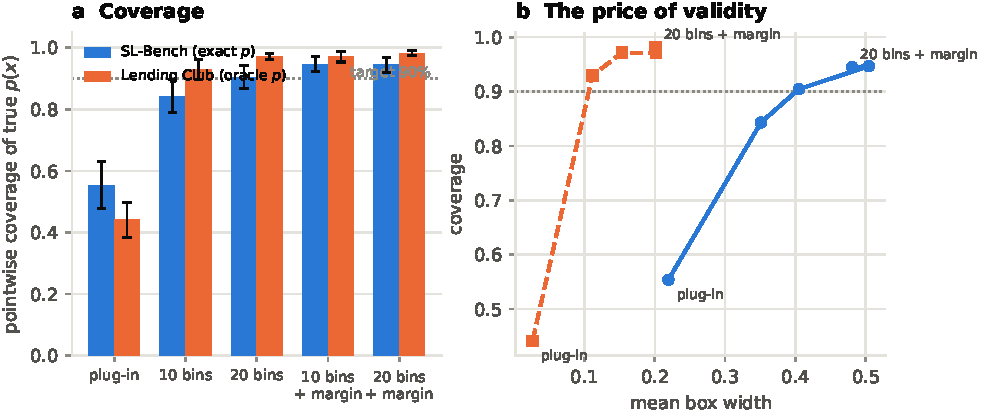
\includegraphics[width=0.8\linewidth]{figures/fig8_nuisance}
\caption{\textbf{Coverage under estimated nuisances} (\cref{thm:nuisance}):
per-unit coverage by construction and the width--coverage trade-off.}
\label{fig:nuisance}
\end{figure}

\subsection{Simulator validation}
\label{app:simulator}

A simulated emergency-department cohort (troponin ordering censors an acute
coronary syndrome label; \texttt{dcl/\allowbreak data/\allowbreak mimic.py}) is used only to check
that the pipeline behaves on a medical-shaped instance with a strong latent
signal; its numbers carry \texttt{data\_source:} \texttt{simulator} and appear nowhere
in the main text. At its $\Gamma_0=\nExpTwoMimicSimGammaZero$ the pattern of
\cref{tab:learning} repeats. Realised risk: ERM-observed
$\nExpTwoMimicSimErmRisk \pm \nExpTwoMimicSimErmRiskCI$, minimax-regret rule
$\nExpTwoMimicSimDclRegThreeRisk \pm \nExpTwoMimicSimDclRegThreeRiskCI$,
oracle $\nExpTwoMimicSimOracleRisk \pm \nExpTwoMimicSimOracleRiskCI$.
Certified regret: $\nExpTwoMimicSimErmRegret$ (ERM) against
$\nExpTwoMimicSimDclRegThreeRegret$ (minimax regret). Observed minus
deployment AUROC: $\nExpTwoMimicSimErmObsMinusTrue$. The above-chance claim
survives to $\Gamma=\nExpFourMimicSimBreakEvenFifty$.

\subsection{The real-data medical arm}
\label{app:medical}

The medical testbed of this paper is the MIMIC-IV-ECG $\times$ MIMIC-IV-ECHO
linkage: the unit is an ECG record, $T=1$ iff the same subject has an
echocardiogram within $\pm365$ days (the EchoNext protocol), restricted to
the echo coverage period, with $Y$ from structured echo measurements (eleven
structural heart disease phenotypes), discharge-summary extraction with a
manually validated sample as fallback, and ICD codes only as an auxiliary
outcome (circular with echo ordering, so appendix-only). The propensity is
estimated from an ECG encoder plus demographics and laboratory values,
cross-fitted and marginalised over the ordering department, and
$\Gamma_{\min}$ is obtained from department-level leniency. The pipeline
(\texttt{dcl/data/mimic\_ecg\_echo}, \texttt{experiments/exp7\_mimic\_ecg\_echo.py})
runs only against the credentialed files on the authors' server and exits
with a distinct error code when any is missing; it never substitutes a
simulator. Its numbers are \textbf{pending} that run and are not reported
here.
